\documentclass{beamer}
\usepackage[latin1]{inputenc}
\usepackage{hyperref}

\usepackage{listings}
\usepackage{color}

\definecolor{dkgreen}{rgb}{0,0.6,0}
\definecolor{gray}{rgb}{0.5,0.5,0.5}
\definecolor{mauve}{rgb}{0.58,0,0.82}

\lstset{frame=tb,
  language=C,
  aboveskip=3mm,
  belowskip=3mm,
  showstringspaces=false,
  columns=flexible,
  basicstyle={\small\ttfamily},
  numbers=none,
  numberstyle=\tiny\color{gray},
  keywordstyle=\color{blue},
  commentstyle=\color{dkgreen},
  stringstyle=\color{mauve},
  breaklines=true,
  breakatwhitespace=true
  tabsize=3
}

\hypersetup{pdftitle={UW Calo Layer1 Tutorial},    % title
    pdfauthor={Bucky},     % author
    colorlinks=true,       % false: boxed links; true: colored links
    linkcolor=red,          % color of internal links (change box color with linkbordercolor)
    urlcolor=blue           % color of external links
}

\usetheme{Warsaw}
\title[UW Layer-1 SW Tutorial]{Layer 1 CaloTrigger Online SW Tutorial}
\author{Bucky Badger}
\institute{UW Madison}
\begin{document}

\begin{frame}
\titlepage
\end{frame}

\begin{frame}[fragile]{How To Make This Document}
\begin{lstlisting}[language=bash]
git clone git@github.com:uwcms/cms-calo-layer1.git
cd cms-calo-layer1/docs
make
\end{lstlisting}
\end{frame}

\begin{frame}{Introduction}
\begin{itemize}
\item This document gives a rough guide to the architecture of the Layer 1 CaloTrigger Online SW
\item Outline
\begin{itemize}
\item oRSC and CTP Architecture
\item IPBus
\item Our "soft" implementation of IPBus
\item VME and SPI byte-stream abstractions
\item Xilinx workflows
\item Existing standalone packages
\item Using XMD to upload and debug SW
\item ToDo list
\end{itemize}
\end{itemize}
\end{frame}

\begin{frame}{Reminder: CTP6/oRSC Architecture}
\begin{itemize}
\item CTP and oRSC have two FPGAs:
\begin{itemize}
\item ``Front end'' is connected to the optical links 
\item ``Back end'' is connected to the world (via VME or Ethernet)
\item FPGAs are connected together via serial bus: UART (CTP6) or SPI (oRSC)
\end{itemize}
\end{itemize}
\begin{center}
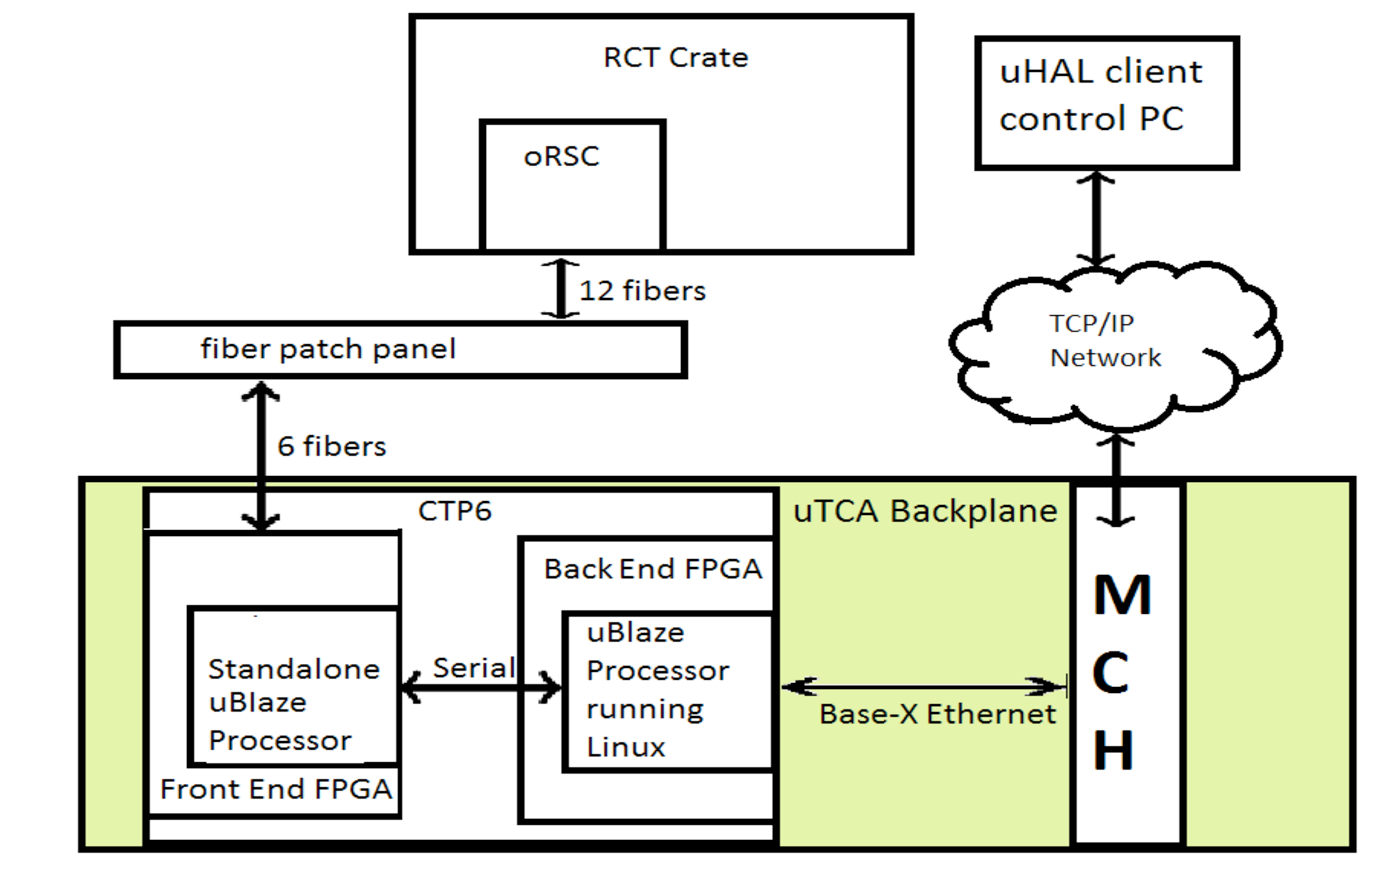
\includegraphics[width=0.7\textwidth]{images/orsc_ctp_ipbus_interface.pdf}
\end{center}
\end{frame}

\begin{frame}{Microblaze \& Petalinux}
\begin{itemize}
\item All of our FPGAs have ``Microblaze'' core
\item This is an (ARM) CPU implemented in HDL
\item On the CTP6 back end FPGA, Linux is installed, so you can SSH in, run multiple programs, etc
\item On all other FPGAs are "standalone". This means you write a C program with a single {\tt int main(void) \{..\}} function
with an infinite loop and this runs everything on the chip
\end{itemize}
\end{frame}

\begin{frame}{IPBus Protocol}
\begin{itemize}
\item Common CMS protocol for interacting with Trigger HW
\item Basically a specification for interpreting ``transactions'' from a byte stream:
\begin{itemize}
\item READ $n$ words (32-bit) from an address in device memory 
\item WRITE $n$ words (32-bit) into an address
\item READ-WRITE-MODIFY at word at an address
\end{itemize}
\item Spec: \url{https://github.com/uwcms/cms-calo-layer1/raw/master/docs/ipbus_protocol_v2_0.pdf}
\item Below: the specification for a READ request/response
\end{itemize}
\begin{center}
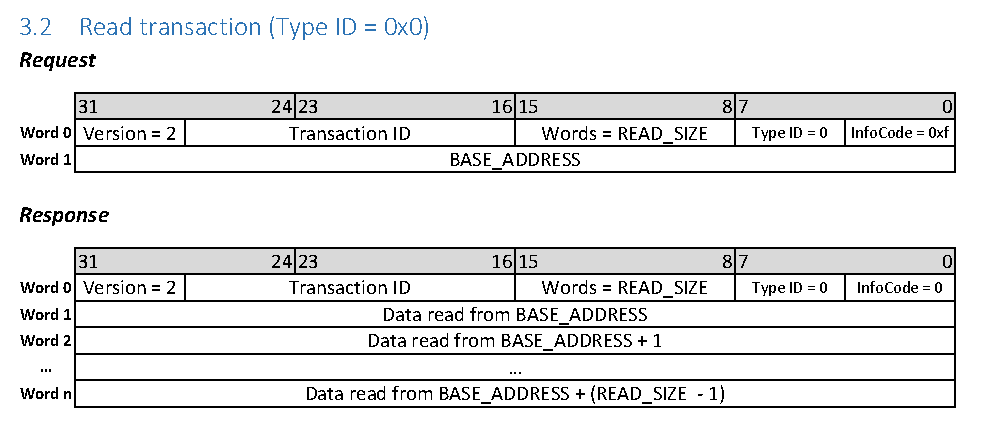
\includegraphics[width=0.8\textwidth]{images/ipbus_read.pdf}
\end{center}
\end{frame}

\begin{frame}{IPBus in C: {\tt softipbus}}
\begin{itemize}
\item Other groups have an HDL core to serve IPBus over UDP
\item We have Microblaze/Petalinux, so we can write C(++) code
\item (and can use the reliable TCP protocol for transport)
\item Our ``softipbus'' implementation is in \href{https://svnweb.cern.ch/trac/cactus/browser/trunk/cactuscore/softipbus}{CACTUS SVN}
\begin{itemize}
\item functions to de-serialize a byte stream into IPBus transactions
\item functions to handle IPBus transactions (READ/WRITE/RWM)
\item functions to serialize the responses into a byte stream
\item a TCP server which runs on Linux and interprets the byte stream as IPBus
\item a TCP server which runs on Linux and forwards the byte stream along a file descriptor
\end{itemize}
\item The code is written so it can run on Linux as a server or used as a library on the standalone devices
\end{itemize}
\end{frame}

\begin{frame}[fragile]{IPBus Clients}
\begin{itemize}
\item The IPBus client $\mu$HAL is made by L1SW group
\item C++ and Python bindings
\item Device memory addresses are mapped to nice names via an XML file
\end{itemize}
\begin{lstlisting}[language=xml]
  <!-- Optical link capture rams -->
  <node id="MGT0" address="0x60000000" size="1024" mode="incremental" permission="r" description="Capture RAM for link #0"/>
  <node id="MGT1"...
\end{lstlisting}
\begin{itemize}
\item CTP6 FE map in CACTUS SVN: {\tt cactuscore/softipbus/etc/ctp6\_fe.xml}
\item CTP6 Python Control Client: \href{https://github.com/uwcms/ctp6commander/blob/master/api.py}{CTP6Commander package}
\end{itemize}

\end{frame}


\begin{frame}{The General Principles}
\begin{center}
{\Large 
Put a softipbus interpreter \\to perform tasks on each FPGA\\~\\
IPBus packets move in a stream of bytes\\~\\
Abstract HW interfaces (VME, SPI, UART) into functions which transport bytestreams
}
\end{center}
\end{frame}

\begin{frame}{Bytestream Abstractions}
\begin{itemize}
\item We want to allow IPBus clients to connect to each FPGA
\item Start with TCP server, which receives a bytestream over ethernet.  This has to live on Linux.
\begin{itemize}
\item TCP server on CTP backend
\item TCP server on "VME PC" connected to the oRSC's crate
\end{itemize}
\item Transport the stream from the server to each FPGA:
\begin{itemize}
\item CTP6 BE - easy, already there (done)
\item CTP6 FE - forward stream from BE server over UART {\tt /dev/tty} (done)
\item oRSC BE - ``VMEStream'' abstracts stream over VME read/write
\item oRSC FE - VMEStream $\to$ oRSC BE $\to$ FE over SPI ("spi-stream")
\end{itemize}
\item Put an IPBus interpreter on each standalone FPGA
\end{itemize}
\end{frame}

\begin{frame}{VMEStream}
\begin{itemize}
\item VME is protocol to READ/WRITE to address in crates - not streaming
\item Goal: transparent continuous bidirectional bytestream over VME
\item Linux VME PC interface:
\begin{itemize}
\item named pipes on filesystem: {\tt mkfifo txbuffer rxbuffer}
\item forward data to oRSC {\tt ./vme2fd txbuffer rxbuffer}
\item {\tt echo "Go badgers" > txbuffer} sends ``Go badgers'' 
\item {\tt cat rxbuffer} prints oRSCs response to stdout
\end{itemize}
\item[] {\bf to forward IPBus over VME:}
\item {\tt softipbus-forward txbuffer rxbuffer} spawns a IPBus TCP server on 60002 and forwards packets to oRSC
\item exact same as on CTP6 BE$\to$FE UART link
{\tt softipbus-forward /dev/ttyUS0 /dev/ttyUS0}
\end{itemize}
\end{frame}

\begin{frame}{VMEStream Protocol}
\begin{itemize}
\item Two RAMS and two registers in memory of oRSC BE
\item Read/write on VME PC via CAEN controller
\item Read/write in oRSC BE standalone code directly from memory
\item Each RAM/register corresponds to a data flow direction
\item When sender has data to send, check if register value is zero
\item If zero, load $n$ words into RAM, set register to $n$
\item Receiver checks of register is $> 0$ - if so:
\begin{itemize}
\item Reads $n$ words of data from RAM
\item Sets register to zero
\end{itemize}
\end{itemize}
\end{frame}

\begin{frame}{SPIStream}
\begin{itemize}
\item oRSC backend and frontend are connected with a SPI
\begin{itemize}
\item Serial Peripheral Interface
\item Master (BE) \& Slave (FE) devices
\item Master always initiates the data interchange
\item Data size is fixed (by Mathias, 512 words)
\end{itemize}
\item https://github.com/uwcms/spi-stream
\item Master continuously initiates exchanges to ensure slave's data is read out 
\end{itemize}
\end{frame}

\begin{frame}{Xilinx Workflows}
\begin{itemize}
\item Three components of a standalone program:
\begin{itemize}
\item HW description XML file - describes HDL devices, memory, etc, built by Mathias
\item Board Support Package (BSP) - generated by Xilinx SDK from HW description XML file. Contains driver header files and libraries for the devices built into the FPGA HDL.
\item Your standalone program. {\tt\#include}s and links to the BSP
\end{itemize}
\item You need to use the Windows (Linux version sorta sucks) Xilinx SDK GUI to generate new BSPs when the HW XML is updated.
\item All other standalone programs are Makefile-ized to prevent tears of blood
\end{itemize}
\end{frame}

\begin{frame}{Existing Standalone Programs}
\begin{itemize}
\item The BSPs, HW, and standalone programs are in Github:
\item \url{https://github.com/uwcms/cms-calo-layer1}
\end{itemize}
\begin{center}
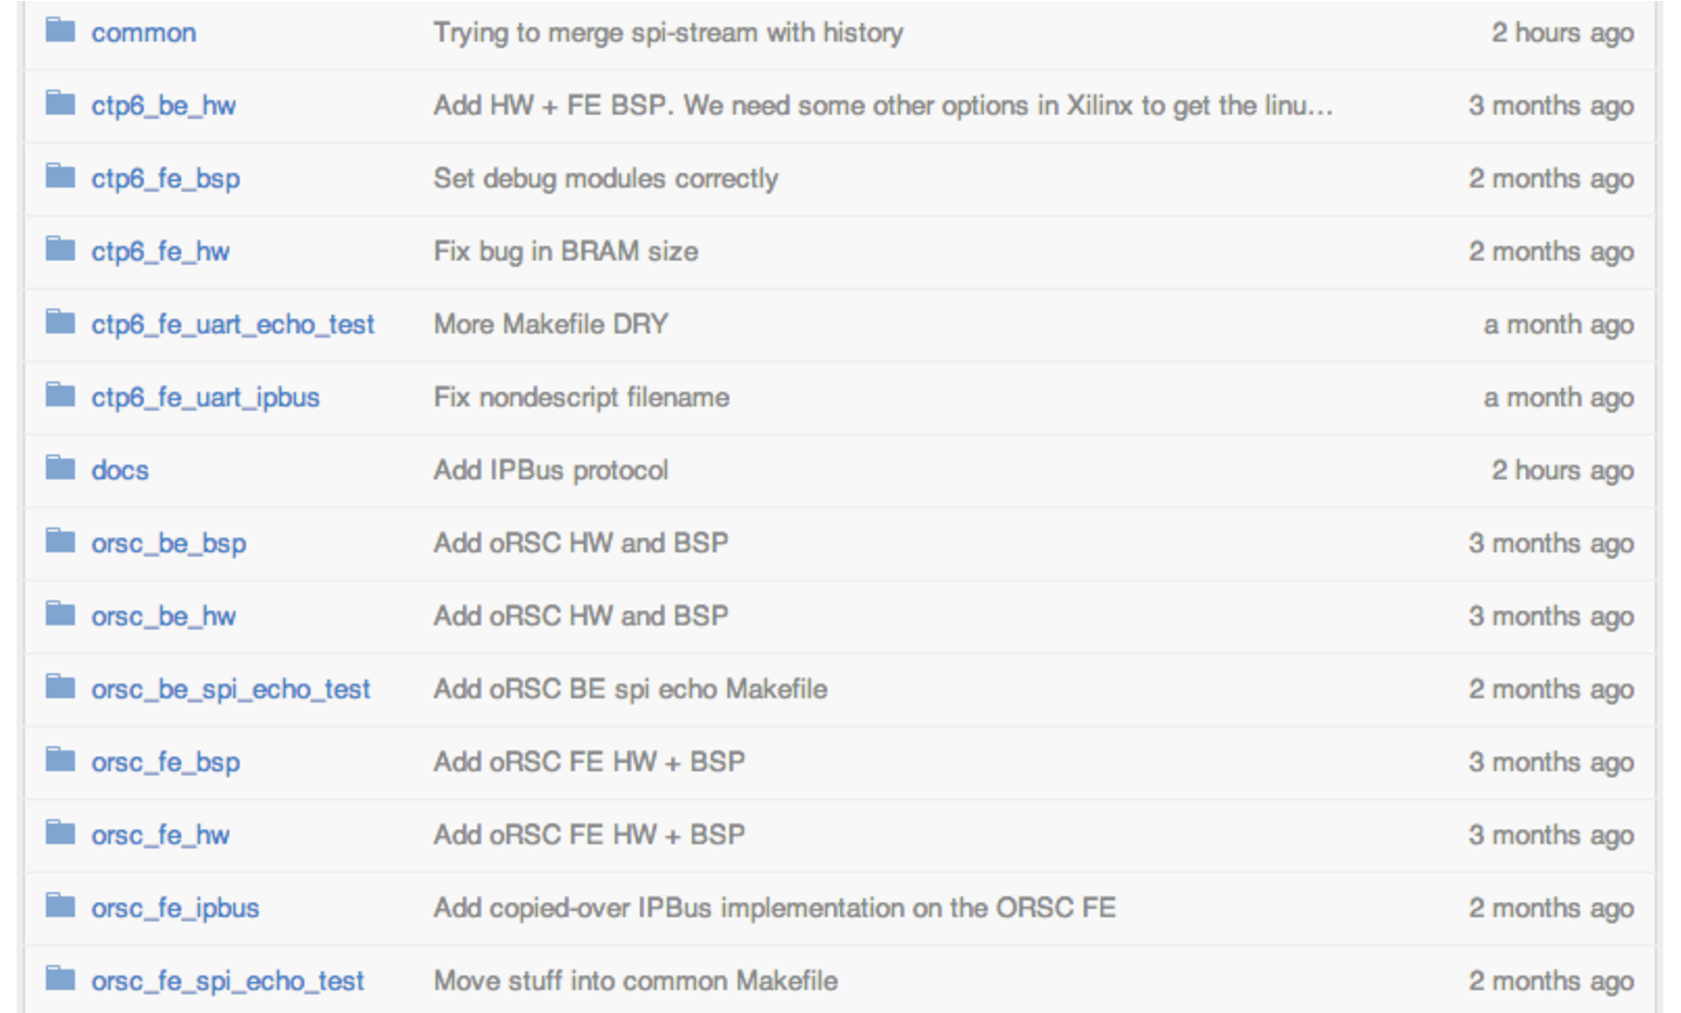
\includegraphics[width=0.9\textwidth]{images/standalone_packages.pdf}
\end{center}
\end{frame}

\begin{frame}{Uploading/Debugging via XMD}
\begin{center}
todo.
\end{center}
\end{frame}

\begin{frame}{Outstanding Tasks}
\begin{itemize}
    \item Update oRSC frontend BSP?
    \item Validate VMEStream with echo test on oRSC backend
    \item Validate SPIStream with echo test between oRSC BE and FE
\begin{itemize}
    \item Code written, needs new BE bitfile(?)
\end{itemize}
    \item Validate IPBus to oRSC FE
    \item Port Tom's bitbanger oRSC backend clock config standalone code
    \item Define (with Mathias) the memory maps for CTP BE, oRSC BE \& FE
    \item Determine what functionality is needed in Supervisor and implement
    \item Write interface for pattern test in oRSC
\end{itemize}
\end{frame}

\end{document}
